\section{3D Renderer}
Doom's 3D renderer is an uncanny combination of proper 3D techniques and screen space tricks. A summary of its main functions (\cw{R\_RenderPlayerView}) reveals it is capable of rendering three things.\\
\par
\ccode{R_RenderPlayerView.c}{}
\par
\begin{itemize}
	\item Segments (walls and portals which are always vertical).
	\item Flats (ceilings and floors which are always horizontal).
	\item Things (also called "masked") which are not only monsters, weapons, ammo, and sprites but also partially-transparent walls.
\end{itemize}
 Its most breathtaking characteristic is its ability to render walls and flats with zero overdraw (each pixel is written exactly once). Sprites and transparent walls do introduce a little bit of overdraw but it is minimal.\\
\par
The life of a 3D frame can be summarized as follows:
\begin{itemize}
\item Render wall segments, sorted front to back from the player's point of view. Both wall ends are projected into screen-space axis X. Based on the distance and floor/ceiling heights of the sectors the wall belongs to, calculate a column Y offset and a height. 
\item To render a full wall, generate a set of columns to make ends meet. Interpolate height and Y vertical columns. While rendering:
   \begin{itemize}
     \item Record screen-space vertical gaps between walls or between wall and screen boundaries. Infer ceiling (if above mid-screen) and floor areas (if below mid-screen) and store the area into an array of structures called "visplanes".
     \item Store sprites to be drawn into an array of structures called "vissprites".
   \end{itemize}
\item Render all ceilings and floors from the visplanes.
\item Render transparent elements and sprites in back-to-front order.
\item Render player sprite (the weapon the Doomguy is holding).
\end{itemize}
\par
The most important part (and what \doom{}'s engine is most famous for) is the ability to sort walls and things extremely efficiently thanks to its Binary Space Partitioning tree. Interestingly, there is a back story about how the BSP came to be a central part of the game engine.\\
\par
\pagebreak



In its earlier versions the engine operated on exactly what the designer produced, namely lines and sectors. Starting in the sector containing the player, the engine would look for double-sided lines and treat them as portals, traversing the map in front-to-back order. Each portal lead to adjacent sectors where the process was repeated recursively.\\
\par
\rawscaleddrawing{0.7}{duke_map}
\par
\vspace{4mm}
In the map above, with the player located in sector \cw{0}, the renderer will flood into other sectors using the red portals. A convex sector \cw{1} is relatively easy to deal with. Things get considerably more complicated when encountering a concave sector like \cw{4}. An even worse case is when nesting occurs like where sector \cw{2} contains another sector \cw{3}.\\
\par
\trivia{The design described is exactly what Ken Silverman's build engine would settle on to power Duke Nukem 3D in 1996. By then the Pentium had taken over the world and was more than able to deal with complex polygons.}\\
\par
\fq{Doom engine was built out of "sectors" -- complex polygonal regions with a common floor / ceiling texture and height, but it didn't have the BSP-chopped "subsectors".  It started in the view sector and recursively flowed into the adjoining sectors, but because they could all be complex polygons it was a lot of record keeping to know what parts you had already visited or were in the stack somewhere.  It worked, and simple areas were fast, but it slowed down precipitously with complexity.}{John Carmack}\\
\par
Things indeed slowed down significantly with a particular map of John Romero's creation.




\fq{I was working on E1M2 around April 1993, and I created a set of circular stairs. John C. wrote the renderer with a sector list to know what should be rendered. The problem is that this set of stairs made his sector list building code take a really long amount of time to execute because the same sectors needed to be put into the list over and over due to how the algorithm worked.}{John Romero}\\
\par
\fullimage{SCREEN01.png}%{Notice the HUD using a huge portion of the 3D canvas.} 
\label{HUD_screenshot}
\par
With the news that their 3D technology was not good enough to ship already a concern, another serious issue arose.\\
\par
Back in August 1992, id Software had landed a contract with Nintendo to port Wolfenstein 3D to SNES. With a release scheduled for May 1st, 1994, they had subcontracted the project and forgotten about it to focus on \doom. In April 1994, the contractor was nowhere to be seen. They had nothing to deliver to Nintendo. It was a big deal involving a huge penalty.\\
\par
 Development for \doom{} stopped immediately as the team desperately banged their old game together into a machine not remotely built to do what they wanted. While Tom Hall dusted off his 6502 assembly skills, John Carmack had a different kind of problem at hand: the raycasting technology which Wolfenstein relied on was too much for the Nintendo console. The SNES and its 6502 on steroids simply did not have enough juice for the DDA algorithm\footnote{You can read everything about DDA in Game Engine Black Book: Wolfenstein 3D.}.\\% It turned out a white paper co-authored by Bruce Naylor would end up making a huge difference.\\
\par



\fq{John started searching around for 3D research papers. He had several VHS tapes of math conferences, and compendiums of graphics papers from conferences because game books were a rare thing back then, and there was nothing printed that could help us create the engine we were building -- he had to figure out where to get information that was not directly applicable to games and figure out how to adapt it to his problem.\\
\par
Bruce Naylor's May 1993 AT\&T Bell Labs paper was titled "Constructing Good Partitioning Trees" and was published in the proceedings of Graphics Interface '93. John had this book in his collection. Bruce's explanation of BSPs was mostly to cull backfaces from 3D models, but the algorithm seemed like the right direction, so John adapted it for Wolfenstein 3D.}{John Romero}\\
\par
\vspace{10pt}
\fq{I do remember clearly that I first used BSP for the SNES version of Wolfenstein, which was a gentle introduction with everything being axial and easier to visualize, which gave me more confidence I would be able to make it work when I went back to working on Doom.}{John Carmack}\\
% Concave and convex sectors proved to be too much complexity for the engine to deal with and maintain a descent frame rate. This was a huge issue. They did not have much time to work on it thought, since around the same time this issue was discovered, work on \doom had to stop in order to respond to an emergency.\\
\par
With a visual surface determination not based on raycasting but rather on BSP, and using a low resolution (112x96 scaled up to 224x192 with Mode 7), Wolfenstein 3D SNES managed to reach an acceptable framerate.\\
\par
Due to Nintendo's strict non-violence policy the game had to be heavily censored to reach a child-friendly quality. Blood was replaced with sweat, guard dogs were replaced with mutant rats, and Hitler was renamed "Staatmeister" (which translates to State Master).\\
\par
With that problem solved, Wolfenstein 3D for Super Nintendo was released on schedule. The whole team resumed cramming for \doom{} and the renderer was changed to also use the power of BSPs.
\pagebreak

\cfullimage{thesis.png}{Bruce Naylor's paper: "Constructing Good Partitioning Trees"}
\pagebreak

\subsection{Binary Space Partitioning: Theory} \label{Binary Space Partitioning: Theory}
Binary Space Partitioning trees have many applications. The one we are interested in is how \doom{} uses them to sort walls rapidly and consistently. Bruce Naylor's thesis paper, "On visible surface generation by a priori tree structures" features a pretty good summary.\\
\par
%  \begin{verbatim}
% In order to determine the visible surface at each pixel,  traditionally
% tile distance from the viewing position to each polygon which maps onto 
% that pixel is calculated. Most  methods  attempt to minimize the number 
% of polygons to be so considered. Our approach eliminates these distance
% calculations entirely.  Rather,  it transforms the  polygonal data base 
% (splitting  polygons when necessary)  into a  binary tree  which can be 
% traversed at image generation  time to yield a visible priority z value
% for each polygon.
% \end{verbatim}

\rawfq{
In order to determine the visible surface at each pixel,  traditionally
tile distance from the viewing position to each polygon which maps onto 
that pixel is calculated. Most  methods  attempt to minimize the number 
of polygons to be so considered. Our approach eliminates these distance
calculations entirely.  Rather,  it transforms the  polygonal data base 
(splitting  polygons when necessary)  into a  binary tree  which can be 
traversed at image generation  time to yield a visible priority z value
for each polygon.
}\\
\par
\fq{When I did the early work on BSPs\footnotemark{}, Bruce Naylor came down and visited here and gave me copies of a bunch of his papers. It's interesting to talk to people about the old days. Of course, you've got the Internet now. You can find anything nowadays. But back then, it was really something to get reprints of old academic papers. There were some clearinghouses I used to use: you'd pay twenty-five dollars or whatever, and they'd mail you xeroxes of old research papers. It was just a very, very different world. I learned most of my programming when I had a grand total of like three reference books. You had to figure everything else yourself. So I was finding I was reinventing a lot of classic things, like Huffman encoding or LZW encoding. So I'd be all proud of myself for having figured something out, and then I'd find it was just classic method and they did it better than I did.}{John Carmack, Interview for Scarydarkfast}\\
\footnotetext{This was during development of Quake; John and Bruce met only after \doom{} had shipped.}
\par
To study BSPs, let's take the example of a map created with DoomED. For simplicity the map we will be working with is made of eight vertices, four linked together to form a room made of four lines (\cw{A}, \cw{B}, \cw{C}, and \cw{D}). Inside the room is a pillar which is also made of four lines (\cw{E}, \cw{F}, \cw{G}, and \cw{H}). The map is made of only one complex sector (it has a hole in it).  Notice that all lines have a direction and all lines have only one side (on their right side). Despite its simplicity it is obvious how it is a difficult problem to solve for a renderer since, depending on the point of view, the order in which the lines/walls must be drawn will vary. A naive solution would require a complex sorting algorithm.\par
\drawing{doom_map}{}
\par
To build the BSP tree from the map, the core idea is to repeatedly select a line to split the map in two. Split lines become \cw{SEGMENTS} and split sectors become {SUB-SECTORS}.\\ 
\par
The choice of the splitter is extremely important. There are good splitters and bad splitters. A list of poor choices for the first splitter would be \cw{A}, then \cw{B}, \cw{C}, and \cw{D} since they would not divide the map evenly.\\ 
\par
Let's say our heuristic selected line \cw{H} which conveniently cuts the room in half. Some lines are entirely to the left of H and some are entirely to its right. Lines on both sides must be split into segments.  After the split, the two leaves in the BSP contain two sub-sectors. One is convex (\cw{\{A, B1, H, D1\}}) and therefore will not be touched anymore. The other one is concave (\cw{\{E, F, G, B2, C, D2\}}) and will need further splitting.\\
\par
 The process is repeated until all subsectors are convex.\\
\par
\drawing{doom_map_split1}{}
\par

Let's follow the process, step by step, until we have a BSP decomposing the space into a set of convex sub-sectors. Notice how, as the binary tree grows, splitter lines are stored in the nodes and segments in the leaves. In the next step, line \cw{G} is selected as the splitter.
\par
\rawdrawing{doom_map_split2}
\par
At this point in the splitting we are still not done. The area between \cw{B2}, \cw{C2}, \cw{E}, and \cw{F} is concave. We need one last split where \cw{F} is selected as splitter.\\ 
\par
\drawing{doom_map_split3}{}
\par
With all sub-sectors in the leaves now convex, the BSP construction ends. The number of vertices and segments to deal with has increased by 50\% but we now have a data structure capable of sorting all segments, from any point of view, at the cost of only three comparisons.\\
\rawdrawing{doom_map_split4}
\par
This is only one of the many possible trees which could have been generated from the map. Choosing splitters in an alphabetical order would have produced an inefficient BSP.\\




\rawdrawing{doom_map_bad}{}
\par

\vspace{-10pt}
\subsubsection{Usage}

\begin{wrapfigure}[10]{r}{0.5\textwidth}
\centering
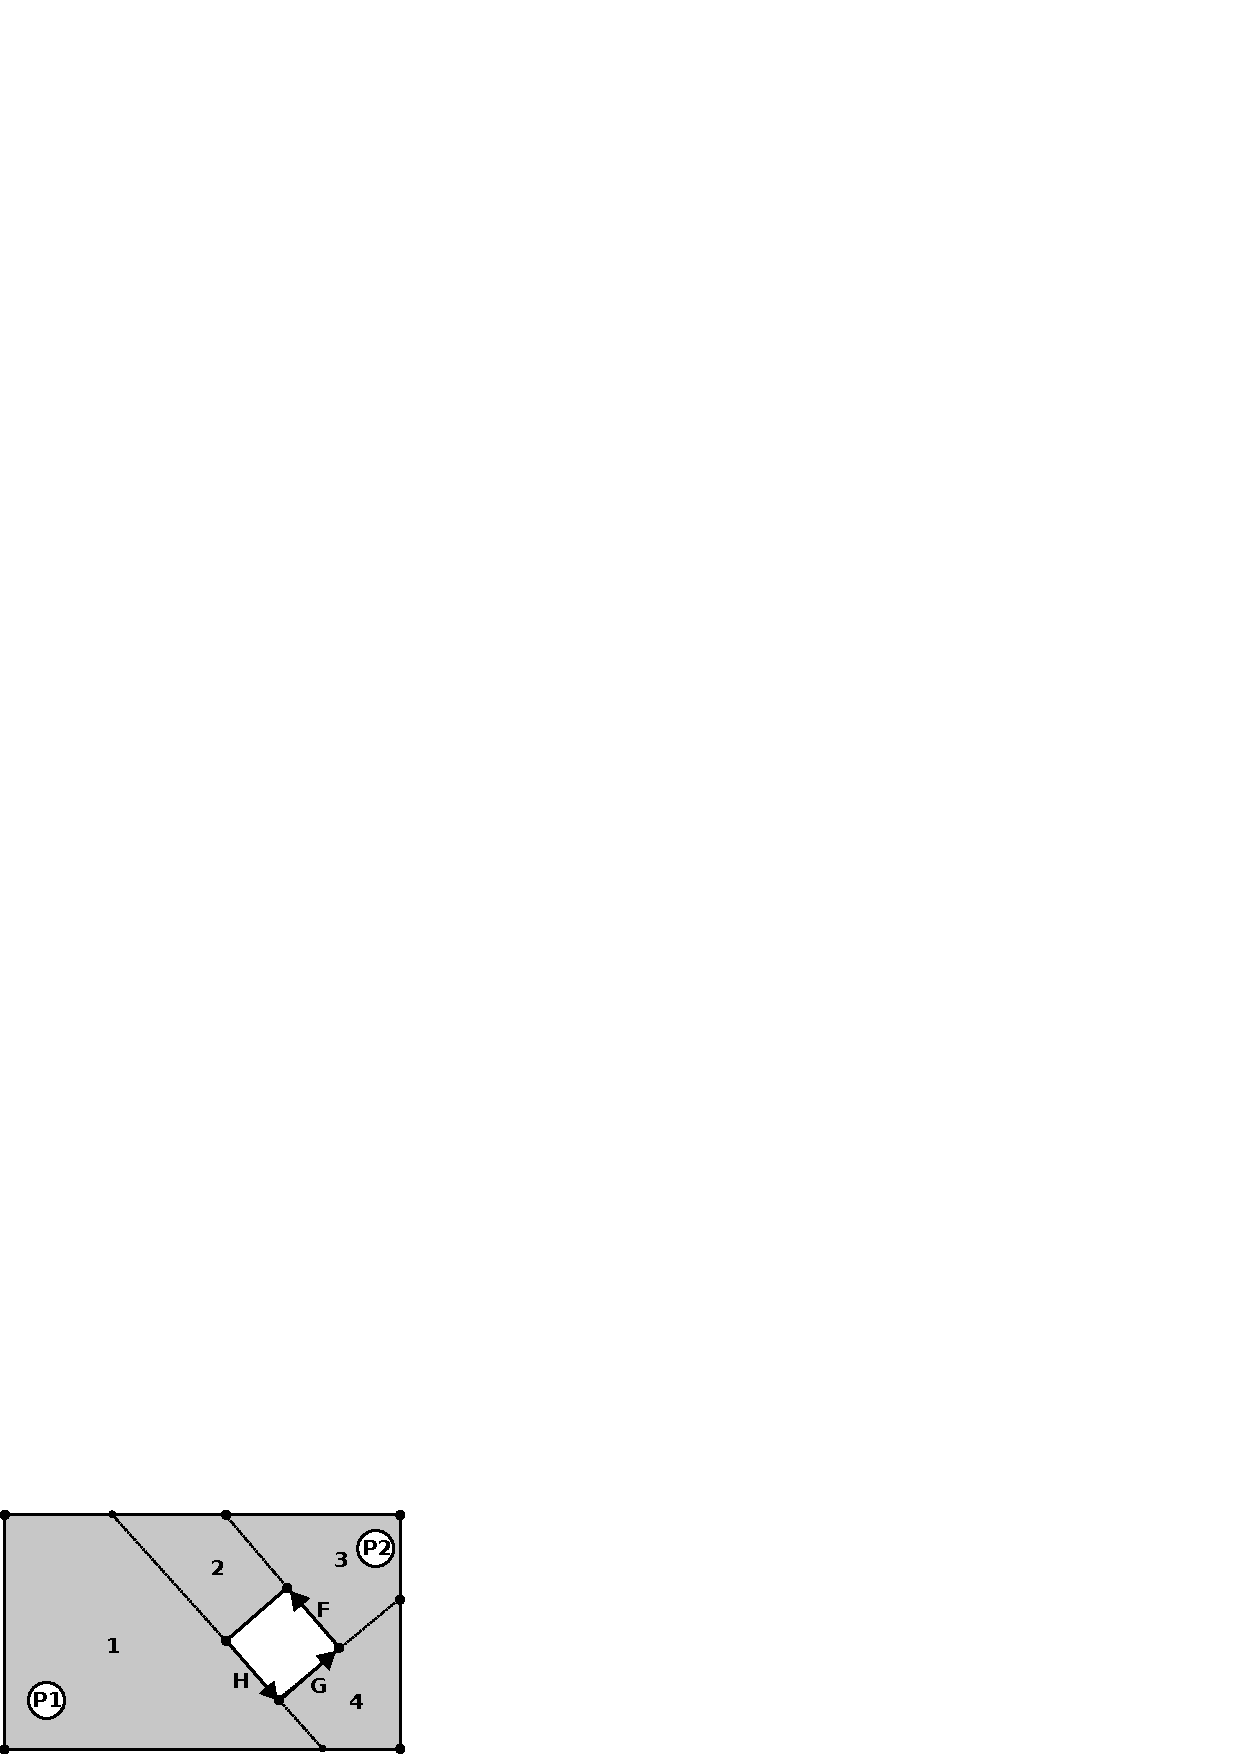
\includegraphics[width=.5\textwidth]{drawings/doom_map_walk.pdf}
\end{wrapfigure}
To use the BSP, we only need to traverse it depth first and choose a branch based on our position in the map. Let's take two examples using the BSP in figure \ref{doom_map_split3} on page \pageref{doom_map_split3}. For convenience of notation, sub-sectors have been labeled \cw{1} to \cw{4} and only the splitting lines are marked.\\
\par
From point of view \circled{\cw{P1}}, traversing the BSP takes three tests. \cw{P1} is on the right\footnote{On the drawing it is on the left but remember that spliting plans have direction (shown via an arrow head). If your turn the page upside down, sub-sector \cw{1} indeed is on the right of \cw{H}} of \cw{H}, on the left of \cw{G}, and on the left of \cw{F}. This gives the front to back order: \cw{1,2,3,4}. Notice that it doesn't matter what order segments within a subsector are drawn since all subsectors are convex.\\
\par
From point of view \circled{\cw{P2}}, traversing the BSP also takes three tests. \cw{P2} is on the left of \cw{H}, on the left of \cw{G}, and on the right of \cw{F}. This gives the near to far order: \cw{3,2,4,1}.\\
\par
The beauty of a binary trees is that traversing it always require the same amount of computation. No matter where we try to place the player on this map, it will always take three tests to sort all subsectors and their segments.
\pagebreak




\subsection{Binary Space Partitioning: Practice}
Maps were preprocessed on a NeXTstation Turbo via the in-house tool node builder named \cw{doombsp}.\\
\par
For the tool to build the best BSP possible a splitter selection heuristic had to be established. A good splitter divides the map as evenly as possible (limiting the depth of the tree), and prefers axis-aligned lines (since they are easier to debug and side tests are faster).\\
\par
 \cw{doombsp} recursively inspects all lines in a subspace and gives a splitting score to each of them. At the end of the evaluation, the highest-scoring line is selected. The map is split in two and the process is repeated until only convex subsectors remain. This is a CPU-intensive task which took eight seconds for E1M1. All thirty maps of \cw{DOOM.WAD} took eleven minutes.\\
\par
\drawing{E1M1_lines}{E1M1, a.k.a Episode 1 Map 1.}
\par
Figure \ref{E1M1_segs} shows the seven first splitters selected on E1M1. The first level is in red, second level in blue and the third level in thick black. Notice how AA splitters are favored.\\
\par
Switching from a sector flooding algorithm to a Binary Space Partitioning algorithm not only added preprocessing time and latency to map designers -- there was another side effect that was more of an issue since it affected players. Because the BSP created new vertices, wall positions are set in stone, there is no way to move walls at runtime.

\drawing{E1M1_segs}{Seven first splitters (three BSP branches) in the E1M1 BSP}
\vspace{5pt}
\drawing{E1M1_fab}{All subsectors at the end of E1M1 tree construction; each is a convex leaf.}

\par


\subsection{Drawing Walls}
With the expert knowledge of BSP in mind, let's take a look at the first step of rendering a scene, namely, wall rendering. As expected, \cw{R\_RenderBSPNode} traverses the binary tree front-to-back. Each sub-sector leaf is sent down to the renderer via \cw{R\_Subsector}.\\
\par
\ccode{R_RenderBSPNode.c}
\par


To perform the side test (\cw{R\_PointOnSide)}, any geometry book will describe how to represent the plane in general form with a vector $(a, b)$ combined to a distance $d$: $$ ax + by + d = 0 $$
Using a dot product operation, the coordinate of the test point $P=(x, y)$ is injected into the plane equation, essentially projecting $P$ onto a line perpendicular to the plane. The sign of the result reveals whether $P$ is in front of or behind the plane (zero = on the plane).\\
\par
This method is far from being optimal. There is a better way, involving neither floating-point nor fixed-point arithmetic, which uses the awesome power of the cross product.\\
\ccode{node_t.c}\\
\par
\vspace{2mm}
\ccode{R_PointOnSide.c}



\begin{wrapfigure}[8]{r}{0.25\textwidth}
\centering
\includegraphics[width=.25\textwidth]{drawings/cross_product.pdf}
\end{wrapfigure}
Notice in the previous code listing how nodes are not stored as coordinates of two vertices (\cw{Point 1}, \cw{Point 2}) but rather as (\cw{Point 1}, \cw{Vector to Point 2}). This storage technique made the cross-product faster to generate since one of the vectors (from the node) was already calculated.\par
\vspace{10pt}


\subsubsection{Wall Projection}
We have now reached the \cw{R\_Subsector} function where all segments in a subsector are rendered in order. This part of the pipeline relies heavily on BAM (Binary Angular Measurement) where degrees in the interval \cw{[0, 360]} are mapped to the full range of a 32-bit integers.\\
\par
\ccode{bam.c}
\par
First, both ends of the segment are converted to an angle with respect to the player's position (via high-school level $angle = arctan(\frac{O}{A})$). Segments with a negative angle (\cw{angle1} - \cw{angle2} < 0) are culled since they are not facing the camera. Segments passing the angle test are then reduced from 32 bits to 13 bits with a simple right-shift. Next, the angle is injected into a lookup table \cw{viewangletox[4096]} to give a screen-space \cw{X} coordinate.\\
 \par
\vspace{2mm}
\drawing{segtobam}{}
\par
Values in \cw{viewangletox} are generated at startup in order to give the player a 90 degree field of view. The table is built such that anything not within 90 degrees is projected onto the edges of the screen. 
\par
\vspace{1cm}
\drawing{angletoxTable}{}
\par
%With the sector floor and height a column dimension and vertical offset are calculated. With the distance to the player, scaling is applied. 
At this point the engine has calculated the screen-space \cw{X} coordinates of both ends of a segment and the distance \cw{z} from the player. But it is not time to draw yet. A little bit of clipping must occur. 






\subsubsection{Wall Clipping}
Here the code branches depending on the two types of segment that can be encountered in a subsector. There are segments with only one side (connected with only one sector) which are opaque and have only a "middle texture". I call these "walls". There are segments with two sides (connecting two sectors) which are often transparent with no middle texture but with an "upper texture" and a "lower texture". I call these "portals".\\
\par
Clipping is a two step process happening in screen space. The first, crude, step is horizontal-based. Only walls affect the horizontal occlusion array but all segments are clipped against it.\\
\par
The second, finer, step is vertically-based. Both walls and portals affect the vertical occlusion array and both are clipped against it.









\subsubsection{Horizontal Crude Wall Clipping}
The first clipping pass is crude and only cares about horizontal occlusion. It maintains a \cw{solidsegs} array which keeps track of the screen-space horizontal occlusion. Since portals can be partially seen through, they have no impact on \cw{solidsegs}. Segments entering this step come out as "fragments" since they may be split due to occlusion.\\
\par
\ccode{hclipper.c}
\par
Let's take a simple example and proceed step-by-step. In the room below, the player is facing north and four walls (\cw{A}, \cw{B}, \cw{C}, and \cw{D}) need to be rendered.\\
\par
\rawdrawing{clip_map}
\par
\vspace{-3mm}
Initially the occlusion array has two entries, one representing what is on the left of the screen, from infinity to -1 and one on the right of the screen from 320 to infinity.
\par 
\begin{minipage}{0.54\textwidth}
\vspace*{2.5mm}
\ccode{clip0.c}
\end{minipage}
\begin{minipage}{0.46\textwidth}
\rawscaleddrawing{0.95}{clip0} 
\end{minipage}
\par






The first wall (\cw{A}) is rendered. There is nothing to occlude it and it is in the middle of the screen. An entry is added to represent the occlusion state.
\par
\begin{minipage}{0.54\textwidth}
\vspace*{2.5mm}
\ccode{clip1.c}
\end{minipage}
\begin{minipage}{0.46\textwidth}
\centering
\rawscaleddrawing{0.95}{clip1}
\end{minipage}
\par



The second wall (\cw{B}) is rendered. Its left side is clamped via angle adjustment and the right side is not occluded. Since it touches the left edge of the screen no entry in the occlusion array is added; only the entry boundaries need to be adjusted.
\par
\begin{minipage}{0.54\textwidth}
\vspace*{2.5mm}
\ccode{clip2.c}
\end{minipage}
\begin{minipage}{0.45\textwidth}
\centering
\rawscaleddrawing{0.95}{clip2}
\end{minipage}
\par





The third wall (\cw{C}) is rendered. It happens to lie just next to the second wall. It is fully converted to a wall fragment and nothing is discarded. The occlusion array is updated.
\begin{minipage}{0.54\textwidth}
\vspace*{2.5mm}
\ccode{clip3.c}
\end{minipage}
\begin{minipage}{0.46\textwidth}
\centering
\rawscaleddrawing{0.95}{clip3}
\end{minipage}
\par


Finally, the last wall (\cw{D}) is rendered. While occluded against the array, it is split into two fragments. The occlusion array is updated. All segments end up touching each other. 
\begin{minipage}{0.54\textwidth}
\vspace*{2.5mm}
\ccode{clip4.c}
\end{minipage}
\begin{minipage}{0.46\textwidth}
\centering
\rawscaleddrawing{0.95}{clip4}
\end{minipage}
\par
\vspace{5pt}
Notice how little RAM was used to maintain the occlusion state and how fast it is to check if the full screen is occluded. All the engine has to do is to check the array is of size 1 and that the range goes from -infinity to +infinity.


\subsubsection{Vertical Fine Wall Clipping}
The second pass is finer and clips vertical segment fragments emanating from the first pass. A data structure based on two arrays as wide as the 3D canvas is maintained. It tracks how much vertical screen-space remains available for each column.\\
\par
 Each rendered segment updates the structure by making increases to \cw{ceilingclip} and decreases to \cw{floorclip}. A column is considered fully opaque when \cw{ceilingclip}'s height and \cw{floorclip}'s height are equal to each other. Wall fragments will mark a column as completely occluded while portal fragments will only update the occlusion columns with what they actually cover in screen-space.\\
\par
\ccode{vclippers.c}
\par
Let's take the example of a simple room made of three sectors (\cw{1}, \cw{2}, and \cw{3}) connected by two portals (\cw{B} and \cw{F}) and surrounded by walls. Sectors \cw{1} and \cw{3} have the same ceiling and floor height but \cw{2} is set to have a higher floor and lower ceiling so that it looks like a window.\\
\par

\begin{wrapfigure}[14]{f}{0.4\textwidth}
\centering
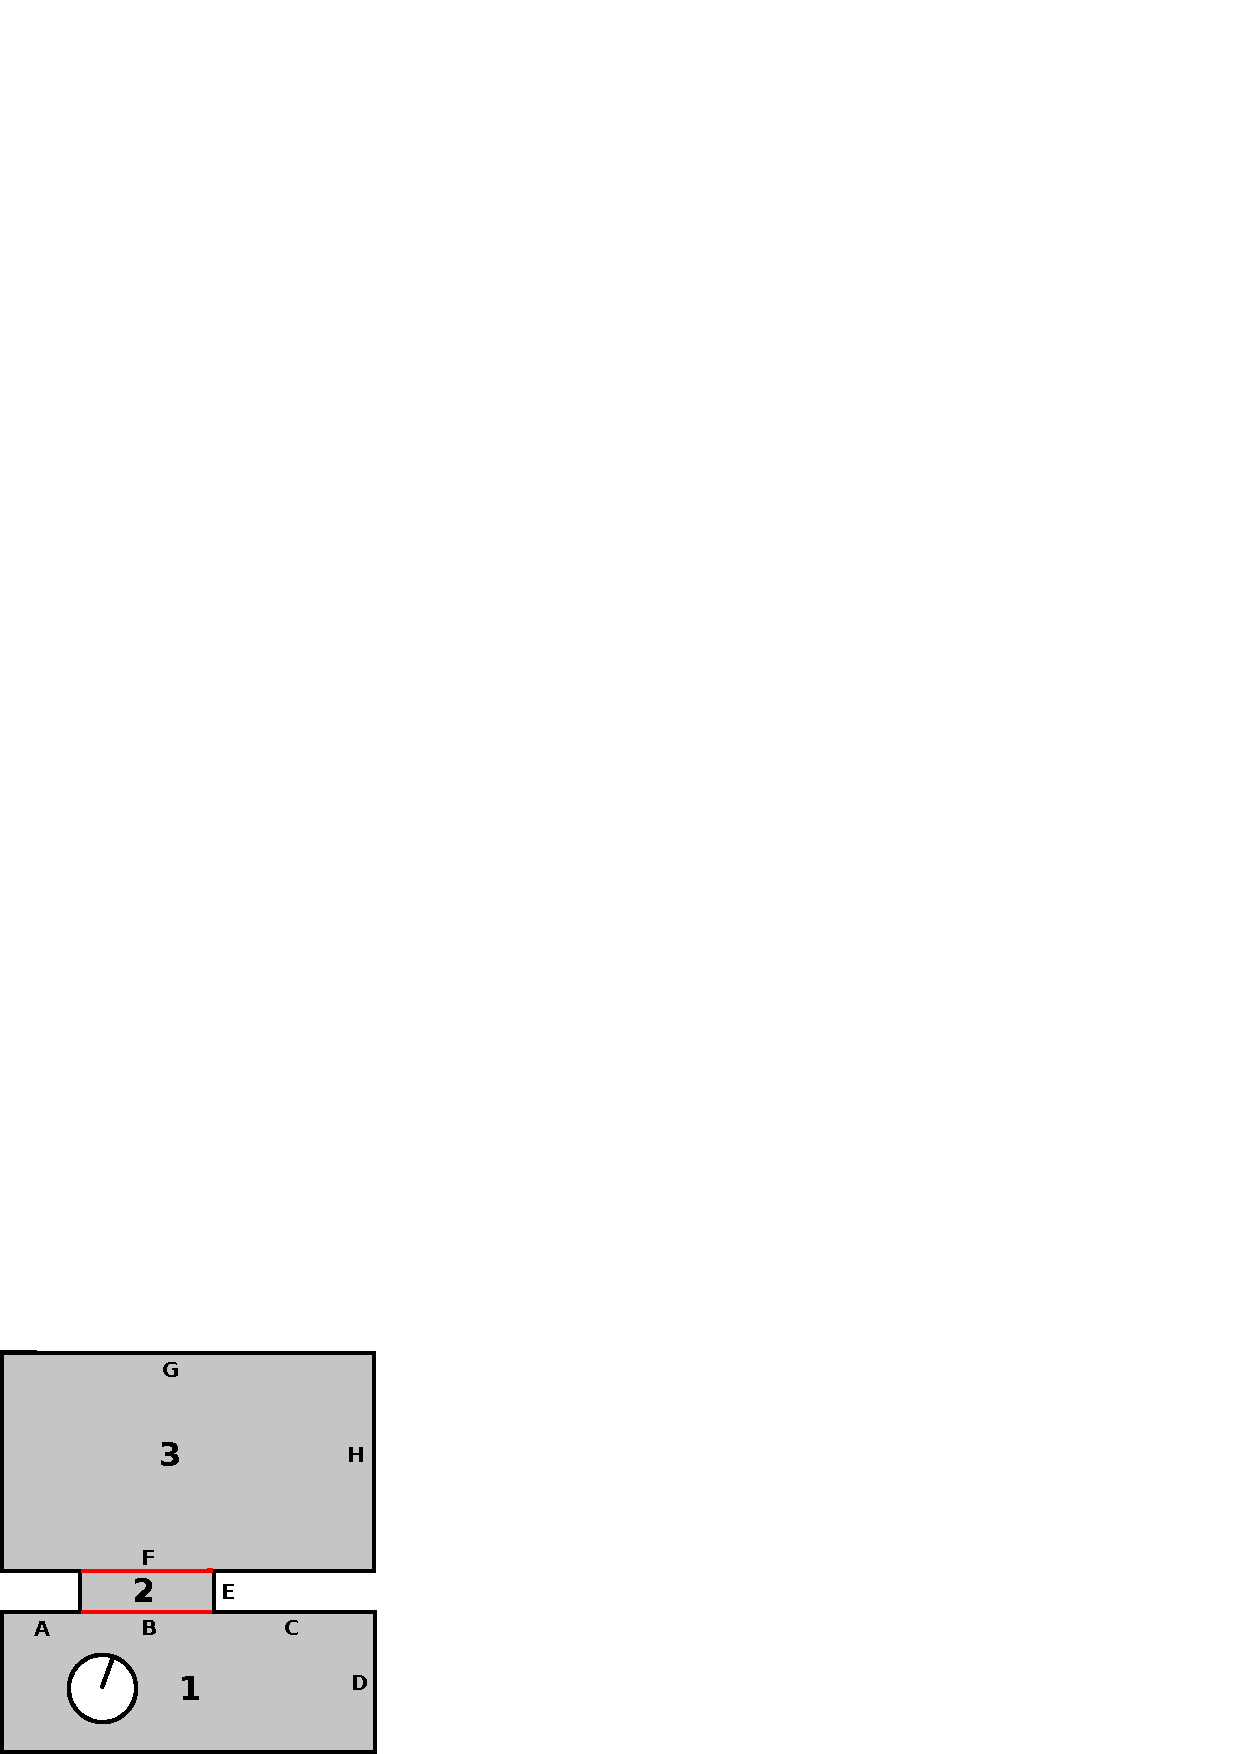
\includegraphics[width=.4\textwidth]{drawings/vcclip_map.pdf}
\end{wrapfigure}
Subsectors are rendered near-to-far in the order \cw{1}, \cw{2}, and \cw{3}. This means segments \{\cw{A}, \cw{B}, \cw{C}, \cw{D}\}, \{\cw{E}, \cw{F}\} and \{\cw{G}, \cw{H}\} (assuming the map was split on lines \cw{B} and \cw{F}). On the opposite page you can see the effect of each wall and portal on the vertical occlusion double array.\par
\vspace{10pt}
Walls \cw{A}, \cw{C}, and \cw{D} mark the full height opaque for each of their columns. The first portal \cw{B} has no middle texture. It is therefore rendered with its upper texture (to accommodate for subsector 2's lower ceiling) and its lower texture (to accommodate for subsector 2 higher floor) and the occlusion array is adjusted accordingly. Wall \cw{E} marks all columns it covers as fully opaque.\\
\par
Notice how portal \cw{F}'s lower and upper textures are not rendered but the occlusion array is still updated. Walls \cw{G} and \cw{H} finish marking the full screen opaque (but were only clipped during the crude pass since they are smaller than the visible window space).


\fullimage{simple_room.png}\\

 \vspace{10mm}


\fullimage{simple_room_clip}














After all this clipping, walls and portal are finally rendered. At the ends of each fragment, a screenspace \cw{Y} offset is calculated based on sector floor, and a column height is generated based on floor/ceiling and distance. These are interpolated to generate a full set of columns of pixels (portals are drawn as a combination of columns according to their upper texture, middle texture, and lower texture while walls only have a middle texture). Rendering is done vertically via the \cw{colfunc} function pointer (detailed in "performance" on page \pageref{performances}).\\

\subsection{Subpixel Accuracy}
It is worth mentioning that the engine is subpixel-accurate when calculating the screen coordinates of a wall's top and bottom edges. Subpixel accuracy is a subtle concept, the advantages of which are best demonstrated with an animated screen. Hopefully a few static drawings will do anyway.\\
\par
 Let's take the example of two points, \cw{A = (0.7, 0.7)} and \cw{B = (5.3, 3.6)} which are to appear on the screen.\\
 \par
\drawing{subpixel}\\
\par
The problem to solve here is: What pixel do you select between \cw{A} and \cw{B}? There are many solutions available here, offering different trade-offs. At the time of \doom{}'s engine, most games discarded the fractional part of a point and then navigated from \cw{floor(A)=(0,0)} to \cw{floor(B)=(5,3)}. This is called "pixel-accurate".\\
\par
Subpixel accuracy is slightly more difficult to perform. Here the fractional part is not discarded but used while navigating from \cw{A} to \cw{B}.\\
\par
Figure \ref{subpixel_before} shows the two methods side by side. The difference looks negligible but it is one of the most important features of the engine which made the world feel "solid".
\drawing{subpixel_before}\\
\par
At first sight it seems the two methods are different yet equivalent, but look at what happens when things start to move, such as in the case where \cw{A} moves \cw{0.3} units down.\\
\par
\drawing{subpixel_after}\\
\par
\vspace{-10pt}
The pixel-accurate method results in five pixels selected differently. The subpixel-accurate way results in one pixel difference. With subpixel accuracy lines tend to be more stable.\\
\par 

\fq{Almost every other texture mapped game back then snapped triangle vertexes to integral pixel values, which meant that the individual texels in a surface would constantly be jumping around by up to a pixel  from even tiny movements.  Basically everything only feels loosely connected, and wiggles around a bit.  DOOM did not have that problem.}{John Carmack}







\subsection{Perspective-Correct Texture Mapping}
Before we move on to how \doom{} drew flats, it is worth noticing that despite using affine texturing to draw columns, the visual result is still perspective-correct.\\
\par
 To illustrate the concept, let's first study what affine texture mapping looks like. We'll use a three-wall-room, each textured with a pattern of white and colored squares.\\
\par

\begin{minipage}{0.43\textwidth}
\rawscaleddrawing{1}{mapping}
\end{minipage}
\hspace{20mm}
\begin{minipage}{0.4\textwidth}

 \scaledimage{1}{square_texture.png} \label{affine_texture_examples}
 \end{minipage}
\par
\vspace{8pt}
In order to focus on walls, the floor and ceiling are intentionally rendered in light gray.\\
\par
\fullimage{affine_texturing.png}
In this scene, wall vertices are projected into screen space coordinates $(x,y)$. A texture coordinate $u$ is generated for each column to draw, based on linear interpolation of screenspace wall width and the column's $x$ coordinate. The texture coordinate $v$ is interpolated linearly based on column height and $y$ position relative to the column. As a reminder, the formula for linear interpolation is as follows:\\
\par
% \begin{figure}[H]
\begin{equation*}
    \scalebox{1.2}{
$u_{\alpha} = (1-\alpha)u_{0}\, +\, \alpha u_{1}\quad{where}\quad0\leq \alpha \leq 1$\\
}
\end{equation*}
% \caption{XXXX}
% \end{figure}
\vspace{3pt}
\par
This texturing technique has the advantage of being fast but has the disadvantage of being visually incorrect. Notice in particular how the "width" of each square is constant even as the wall columns get further away. In order to generate correct texture coordinates, the $u$ coordinate needs to factor in the distance from the player. To this effect, value $\frac{1}{z}$ (which is linear in screen space) is used:\\

% \begin{figure}[H]
\begin{equation*}
    \scalebox{1.2}{
$u_{\alpha} = \dfrac{
                      (1 - \alpha)\dfrac{u_{0}} {z_{0}} +    \alpha\dfrac{u_{1}} {z_{1}}  
                    }       
                    {  
                      (1 - \alpha)\dfrac{1} {z_{0}} + \alpha\dfrac{1} {z_{1}}    
                    }   \quad{where}\quad0\leq \alpha \leq 1 $\\
}
\end{equation*}
\par
\vspace{4pt}
The calculation is much more expensive but now the result is perspective correct.\\
\par
\fullimage{perspective_texturing.png}
Had \doom{} allowed sloped walls, texturing would have required six perspective correct computations per pixel (both $u$ and $v$ interpolated twice along vertical and horizontal edges of a quad) which would have been prohibitively CPU intensive.\\
\par
 By enforcing walls to be strictly vertical, \doom{} was able to perform the expensive perspective correct computation only once per pixel column, use linear interpolation to draw each column, and still yield a visually correct result. It works because along a column, the distance from the player is constant. This trick effectively managed to produce perspective correct texture mapping at the computational cost of affine texturing.\\
\par
Given the previous screenshots, it may not be clear why perspective correctness is so important and why the engine goes to such an extent just to be "correct". Keep in mind these were just examples to demonstrate the problem. As soon as real textures are used (using \doom{}'s marble textures featured below), the visual disturbance cannot be ignored.\\
\par
\par
\begin{minipage}{0.32\textwidth}
\cfullimage{MWALL4_1.png}{\cw{MWALL4\_1}}
\end{minipage}
\hspace{1mm}
\begin{minipage}{0.32\textwidth}
\cfullimage{MWALL4_2.png}{\cw{MWALL4\_2}}
\end{minipage}
\hspace{1mm}
\begin{minipage}{0.32\textwidth}
\cfullimage{MWALL5_1.png}{\cw{MWALL5\_1}}
\end{minipage}
\par

On the opposite page, notice in particular how \cw{MWALL4\_1}'s upper right pentagram edge appears arched instead of being straight. The same thing happens with \cw{MWALL5\_1} where the left horn does not look right. \cw{MWALL4\_2} suffers none of these issues since it is parallel to the viewing angle.\\
\par
Several video game consoles of the era such as the PlayStation, the 3DO, and the Saturn\footnote{Thanks to a close collaboration with SGI, Nintendo gifted the Nintendo 64 with perspective correct texturing which made Zelda and Mario look amazing.} featured hardware accelerated graphics but not perspective correctness. On these machines, affine texture mapping artifacts were supposed to be compensated for either via triangle sub-divisions or by avoiding texturing altogether. This is why PSX game \textit{Crash Bandicoot}'s characters are devoid of texturing in favor of Gouraud shading.\\
\par
John Carmack hated affine texturing so much he vetoed all ports attempting to be perspective incorrect which sometimes resulted in serious consequences (page \pageref{saturn_port}).\par



\fullimage{game_affine_texturing.png}
\par
\vspace{5pt}
% \fq{The book "Fundamentals of Interactive Computer Graphics" was my bible in the late 80's. I tried to make the cover image\protect\footnotemark on my //GS, but I didn't grok perspective correct texturing.}{John Carmack}\\
% \footnotetext{An exploded texture-map cube for which perspective correctness is paramount.}
Above, distorted walls due to affine texturing. Below, perspective correct texturing.\\
\par
\fullimage{game_perspective_texturing.png}

\vspace{-30pt}
\subsection{Drawing Flats}
 If we were to take a look at the framebuffer at this point in the rendering of a frame, it would look like mashed potatoes (see opposite page where flats are in white to ease visualization). \doom{} never clears the framebuffer so instead of white there would be whatever was drawn last frame.\\
\par
To render the flats, the engine uses a data structure generated while the walls and portals were being rendered. These are called "visplanes".\\
\par
\ccode{visplanes.c}\\
\par
The concept of visplanes is the most difficult aspect of \doom{} to understand. The comments in the source code manifest their esoteric nature and also attest that even people closely related to id Software did not fully grasp what they were.\\
\par
A visplane describes a screen-space area representing either a ceiling or a floor. It has a height, a texture (\cw{picnum}), and a light level. To describe the limits of its area, it has two arrays as wide as the screen. Areas are represented as a set of columns with one column possible per \cw{X} coordinate.\\
\par
\trivia{The engine stores visplanes before drawing them. If storage runs out, the engine terminates execution and returns to DOS with a less than useful error message.}\\
\par
\fakedosoutput{no_more_visplanes.txt}

\fullimage{mashed_potatoes1.png} \label{mashed_potatoes1.png}

Above is the final frame. Below is the current state of the frame with missing visplanes.

\vspace{4mm}
\fullimage{mashed_potatoes2.png}
Visplanes represent the vertical "gaps" in screen-space between fragments and screen borders or between walls and portals. To better understand how they are generated, let's take an example and go back to the simple room we just studied. This time we will focus on how the \cw{visplanes} array is populated.\\
\par

\begin{wrapfigure}[16]{r}{0.45\textwidth}
\centering
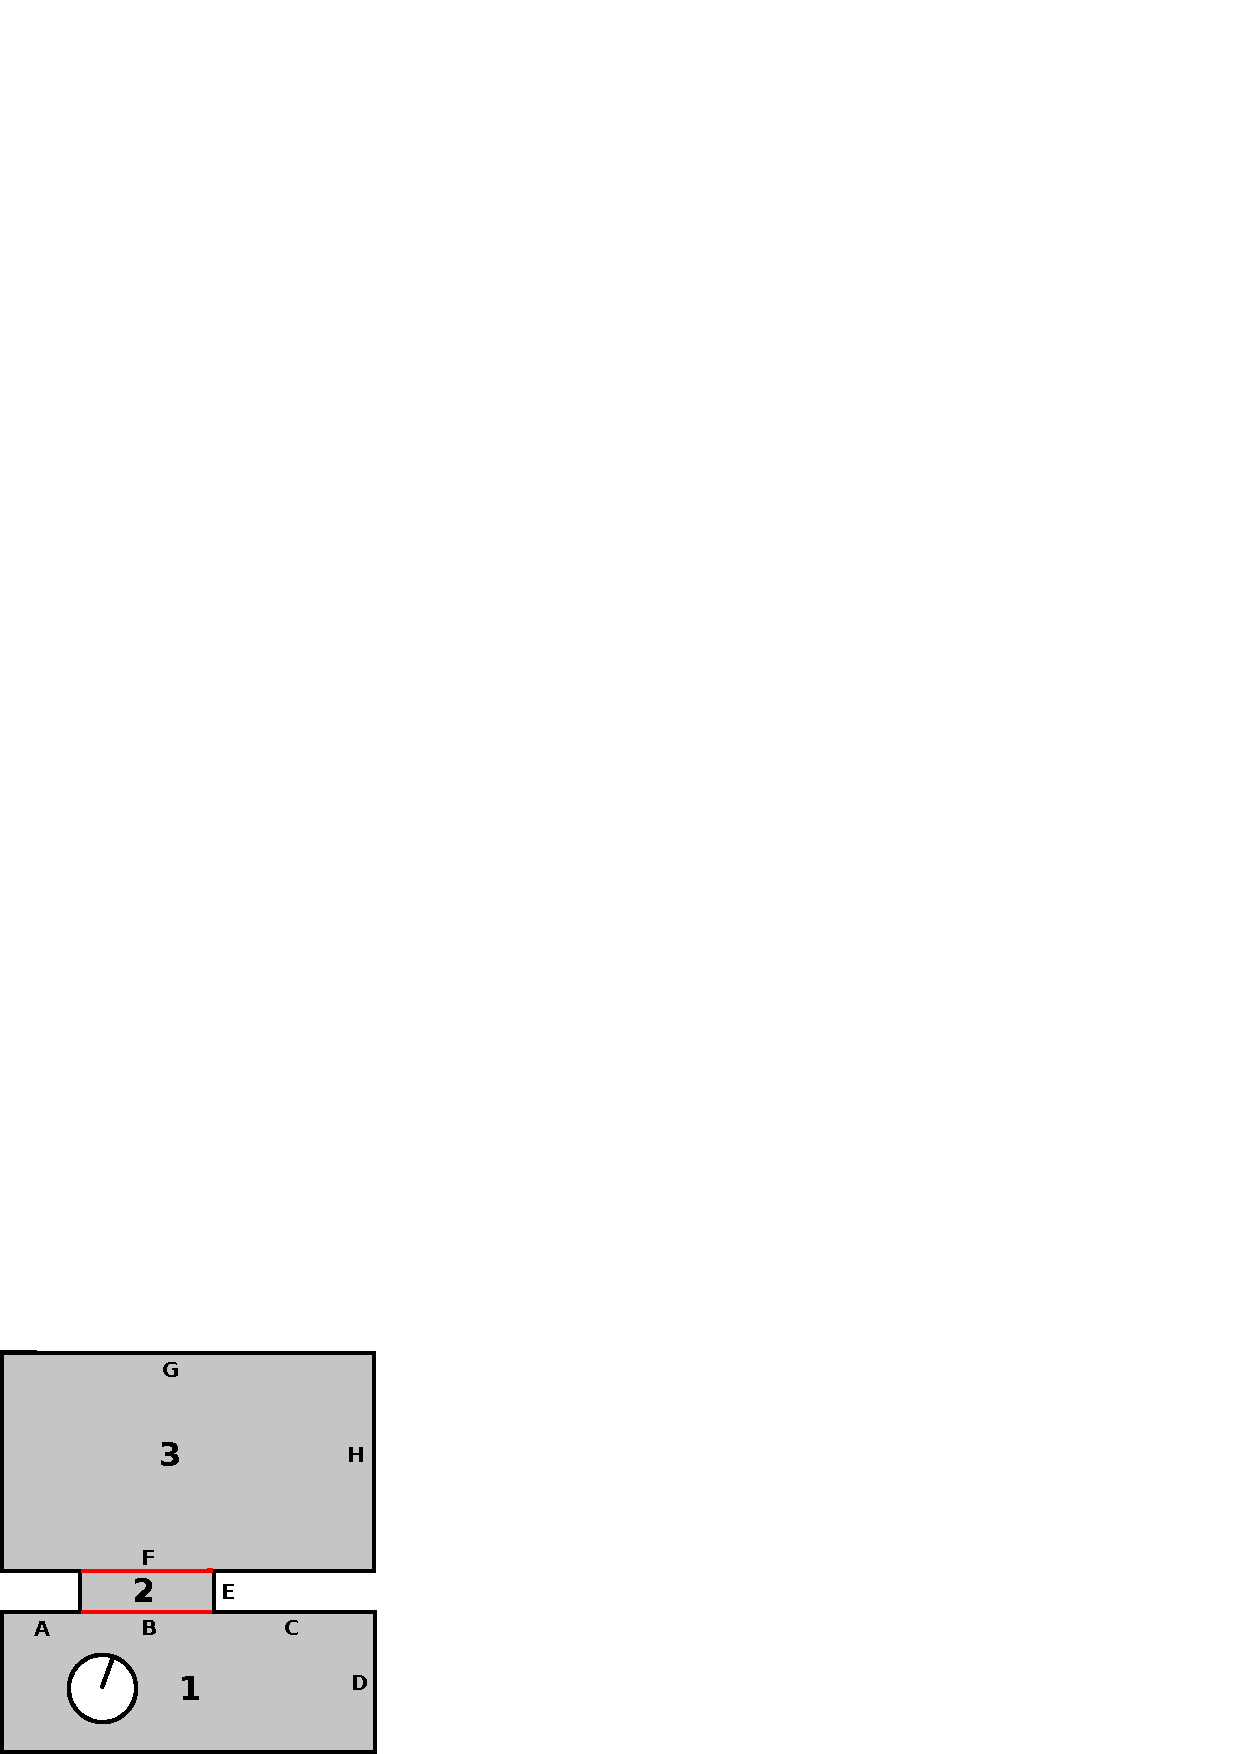
\includegraphics[width=.45\textwidth]{drawings/vcclip_map.pdf}
\end{wrapfigure}
As in the previous example, sectors are rendered near to far, resulting in segments in the following order: \cw{A}, \cw{B}, \cw{C}, \cw{D}, \cw{E}, \cw{F}, \cw{G}, and \cw{H}.\\
\par
When wall \cw{A} is rendered, it is clipped horizontally and vertically. Since it uses all the vertical screen space, no visplanes are created.\\
\par
 Things get slightly more interesting when walls \cw{C} and \cw{D} are rendered. Since they do not occupy the full height (there is a gap between the screen and the top/bottom edge of the walls), two visplanes are created per fragment -- (\cw{1},\cw{2}) and (\cw{3},\cw{4}) -- and stored in the visplane array.\\
 \par
  Likewise, when portal \cw{B} is rendered, there are gaps above its upper texture and below its lower texture, so two additional visplanes (\cw{5} and \cw{6}) are added.\\
\par
Wall \cw{E} is another new case. The gaps above and below are not between a wall and the screen but between  \cw{E} and portal \cw{B}'s upper and lower parts. To detect the previous boundaries, the previously-seen vertical occlusion array is used to create visplanes \cw{7} and \cw{8}.\\
\par
Portal \cw{F} is yet another special case. Since from this point of view it is connecting to a sector with a higher ceiling and a lower floor and has no middle texture, nothing is rendered. Yet the coordinates of its middle part are still generated in order to generate visplanes \cw{9} and  \cw{10}.\\
\par
From this point on, the process is repeated. Wall \cw{G}'s rendering generates visplanes \cw{11} and  \cw{12} and wall \cw{H}'s rendering generates visplanes \cw{13} and  \cw{14}.\\
\par
The visplane generation algorithm is quite simple. However it generates many visplanes and therefore consumes a lot of RAM. To address this issue, \doom{} merges visplanes.\\
\par
\trivia{The \cw{visplane\_t} struct requires 664 bytes per visplane. The engine reserves space for 128 visplanes. The total represents a significant amount of RAM (84,992 bytes) accounting for roughly two percent of the minimum required (4MiB).}








\fullimage{simple_room_visplanes}

\vspace{4pt}

Below, the engine was modified to draw walls and flats in plain color to show merging.

\vspace{5pt}
\fullimage{small_room_visplanes.png}




\fullimage{complex_scene_plain_light.png} \label{complex_scene_plain_light.png}

% \vspace{3mm}


E1M1 benefits from merging. Reproduced below without diminished lighting for clarity.

\vspace{2mm}
\fullimage{complex_scene_plain.png}



\fullimage{complex_scene_multivis.png}

% \vspace{3mm}

Without merging (above) the frame requires 179 visplanes. With merging (below), only 28 are needed.

\vspace{2mm}
\fullimage{complex_lowvis.png}\par \pagebreak
On the previous page, the modified engine shows how a visplane does not need to be horizontally continuous. The red floor's visplane for example is made of three parts yet uses only one entry in the visplane array, validating the judicious choice to represent visplanes as an array of columns.\\
\par
There are several conditions required to merge two visplanes. Mergeable visplanes must have the same height, light and texture. Even if these conditions are met, the data structure has to be able to absorb others. This is only possible if visplanes are side-by-side. Even one pixel above or below with the same \cw{X} coordinate makes two visplanes ineligible for merging. Function \cw{R\_FindPlane} looks for candidates; mergability is tested elsewhere.\\
\par
\ccode{visplane_linear_search.c}
\par
Notice the overflow check which was mentioned earlier. This case was a map designer's worst nightmare since its meant abrupt termination without much information provided to fix the error. Many legends and theories circulated until the source code was released\footnote{"The Facts about Visplane Overflows" by Lee Killough}.





\subsection{Drawing Flats (For Real)}
We can finally read the flat drawing routine which iterates over the array of visplanes.\\
\par
\ccode{R_DrawPlanes.c}
\par
Notice how the flat texture resource is not freed at the end of each iteration but rather marked as \cw{PU\_CACHE} according to what was described in the memory manager section.\\
\par
Despite being stored as columns, visplanes are converted to horizontal spans. Rendering this way allows for fast perspective correct texturing since each line is at a constant distance from the player.
% Since distance from the player is constant over a horizontal line, visplanes are rendered as spans (instead of columns) for perspective correctness. 
This choice also allowed fast rendering of something we have so far ignored: diminished lighting.






\trivia{The limitation of 128 visplanes was not only necessary to fit within the memory budget, it was also a runtime necessity. When attempting to merge visplanes, the engine searches linearly, making it a $O(n})$ operation which would become a bottleneck as the number of visplanes increased. In 1997, Lee Killough lifted this limitation, replacing linear search with a $O(1)$ chained hash table\footnote{Source: "The Truth about Visplane Overflows".}.




























\subsection{Diminishing Lighting}
\label{diminishedlightning}
\begin{wrapfigure}[11]{r}{0.33\textwidth}
\centering
\scaledimage{0.33}{palette.png}
\end{wrapfigure}
So far, in order to introduce complexity gradually, our trip down the rendering pipeline has completely ignored diminishing lighting. It was assumed that texel values from texture and sprite were used as-is and written directly to the framebuffer. Now it is time to introduce the concept of lightmaps.\\
\par
In order to convey a scary atmosphere, \`a la Aliens, it was decided from day one that with increasing distance, colors would fade to black. Map designers also wanted to be able to switch the light in a room on and off and also to dim it if necessary. In response to this requirement, the engine had to be able to draw shades of color. With the VGA system limited to 256 colors from a palette, a possible implementation would have been to restrict artists to use 16 colors and use the 240 other slots to generate 15 shades of each "primary" color.\\
\par
This would have severely impaired the work of the artists, not to mention it would have looked poor during outdoor scenes where light is not diminished with distance. Once again a clever trick allowed artists to use the full 256 colors for their assets and not 16 but 32 shades of the same color. On paper that would have meant $256 * 32 = 8192$ colors which the VGA hardware did not support.\\
\par
 The trick to fake more colors than available is to use an indirection "light table" where the other 255 colors are used to approximate a gradient for each of the 256 entries. The lightmap is 256 entries tall (one for each index) and 32 wide (one column for each shade). In figure \ref{COLORMAP.png} you can see how the original palette lines are unrolled vertically in the left-most column (notice the isolated white at the top and the pink at the bottom). Each row is a 32 value gradient toward black, using the same 256 colors. The right-most column is all black. The trick has its limits. It works well for red but not too well for crimson and yellow.\\
 \par
 To use the lightmap, take the original texel value \cw{T} which is between [0,255]. This will be the \cw{Y} coordinate. Take a light value \cw{L}, with 0 being the brightness and 31 being the darkest. This will be the \cw{X} coordinate. The value to write in the framebuffer is \cw{lightmap[X][Y]}.\\
 \par
\cscaledimage{1}{COLORMAP.png}{The \cw{COLORMAP} contains 32 shades of 256 colors yet still 256 colors total.}





\fullimage{diminishedlight2.png}

Above shows the vanilla engine (with thing rendering disabled). Below is the same scene with a modified lightmap-less engine.
\vspace{2mm}

\fullimage{diminishedlight1.png}
\vspace{-10pt}
\cfullimage{diminishedlight3.png}{Same scene as opposite page, with lightmaps but with texturing disabled.}
\par
The visual effect of lightmaps can sometimes be subtle. On the opposite page, a normal scene (above) shows no banding. Disabling lightmaps altogether (opposite page, below) makes the colors appear washed out. Disabling texturing by rendering walls in white (\cw{0x04}) and flats in brown (\cw{0x80}) (as in figure \ref{diminishedlight3.png}) makes lightmaps and banding vividly apparent.\\
\par
Because calculating which lightmap to use is based on the distance from the player and also on the sector light level, it is a slightly expensive operation.\\
\vspace{10pt}
\begin{equation*}
    \scalebox{1.2}{
$lightmapId = sectorLightLevel + z * diminishingFactor$\\
}
\end{equation*}
\par
\begin{equation*}
    \scalebox{1.2}{
$   color = lightmapId[textureTexel] $
}
\end{equation*}
\par
\vspace{10pt}
 % To reduce lightmap arithmetic, the scene drawing is dictated by where the lightmap value is constant. Therefore, walls are drawn as columns and flats are drawn as lines. 
 In scene where a lot of visplanes are on screen, even selecting the proper lightmap ID was a performance hit. Therefore, a cache system keeping track of lightmap ID on a per screenspace line/sector ID mitigate how often the value is calculated.\\% Since a visplane can be horizontally discontinue, \\
 \par
 The engine uses a cool trick to embellish orthogonal surface rendering. Lightmap selection is tweaked based on world-space orientation. For north-south walls, the selection is lowered by one unit, making them brighter. For east-west walls the lightmap selection is increased by one unit, making them darker. Lightmap selection on other walls is unaffected.\\



To render the sky, a sector has a special ceiling texture number which the engine recognizes as "sky", in which case its height is 0, lightmap is 0 and perspective is disabled. Each portion of the sky is stored as a visplane and drawn as a column of pixels (with \cw{colfunc}).\\

\par
The \cw{COLORMAP} contains a 32nd lightmap made of 256 shades of grey. It is used when the player picks up the invulnerability bonus. There is a bug in the visplane rendering routine's special casing that handles skies. Skies are always renderered without diminished lighting and therefore ignore lightmaps.\\
\par
 This causes a weird visual result when a player is outside and picks up the invulnerability orb, where everything except for the sky is rendered with a shade of gray.\\
\par 
% \ccode{lightmap.c}
% \par
\fullimage{invulnerable.png}\\
\par
The effect was diffcult to replicate with seemingly "more powerful" hardware accelerated systems which use 24-bit colors. On iOS, \cw{glBlendFunc(GL\_ONE\_MINUS\_DST\_COLOR, GL\_ZERO)} was used to approximate the same visual with mixed results.\\
\fullimage{idbeholdv.png}\\
\par
Above is the invulnerability effect as it appeared on the PC version. Below, how it was done on iOS via OpenGL ES 1.0 \cw{glBlendFunc} function.\\
\par
\fullimage{invOpenGL.png} 














\subsection{Drawing Masked}
With the environment rendered, what remains are "masked" elements. This category encompasses not only all sprites but also partially-transparent walls and the player's weapon.\\
 \par


\scaledimage{0.25}{cacodemon1.png}\scaledimage{0.25}{cacodemon2.png}\scaledimage{0.25}{cacodemon3.png}\scaledimage{0.25}{cacodemon4.png}\\

\scaledimage{0.25}{cacodemon9.png}\scaledimage{0.25}{cacodemon10.png}\scaledimage{0.25}{cacodemon11.png}\scaledimage{0.25}{cacodemon12.png}\\

\scaledimage{0.25}{cacodemon17.png}\scaledimage{0.25}{cacodemon18.png}\scaledimage{0.25}{cacodemon19.png}\scaledimage{0.25}{cacodemon20.png}\\

\scaledimage{0.25}{cacodemon25.png}\scaledimage{0.25}{cacodemon26.png}\scaledimage{0.25}{cacodemon27.png}\scaledimage{0.25}{cacodemon28.png}\\
\pagebreak


The function responsible for this task is called \cw{R\_DrawMasked}. It is the last step in the rendering pipeline. Contrary to the environment which is rendered in front-to-back order, this step proceeds in back-to-front order (which is the only way to get transparency right).\\
\par
\vspace{2.3mm}
\scaledimage{0.25}{cacodemon5.png}\scaledimage{0.25}{cacodemon6.png}\scaledimage{0.25}{cacodemon7.png}\scaledimage{0.25}{cacodemon8.png}\\

\scaledimage{0.25}{cacodemon13.png}\scaledimage{0.25}{cacodemon14.png}\scaledimage{0.25}{cacodemon15.png}\scaledimage{0.25}{cacodemon16.png}\\

\scaledimage{0.25}{cacodemon21.png}\scaledimage{0.25}{cacodemon22.png}\scaledimage{0.25}{cacodemon23.png}\scaledimage{0.25}{cacodemon24.png}\\

\scaledimage{0.25}{cacodemon29.png}\scaledimage{0.25}{cacodemon30.png}\scaledimage{0.25}{cacodemon31.png}\scaledimage{0.25}{cacodemon32.png}\\

\pagebreak






\begin{wrapfigure}[12]{r}{0.5\textwidth}
\centering
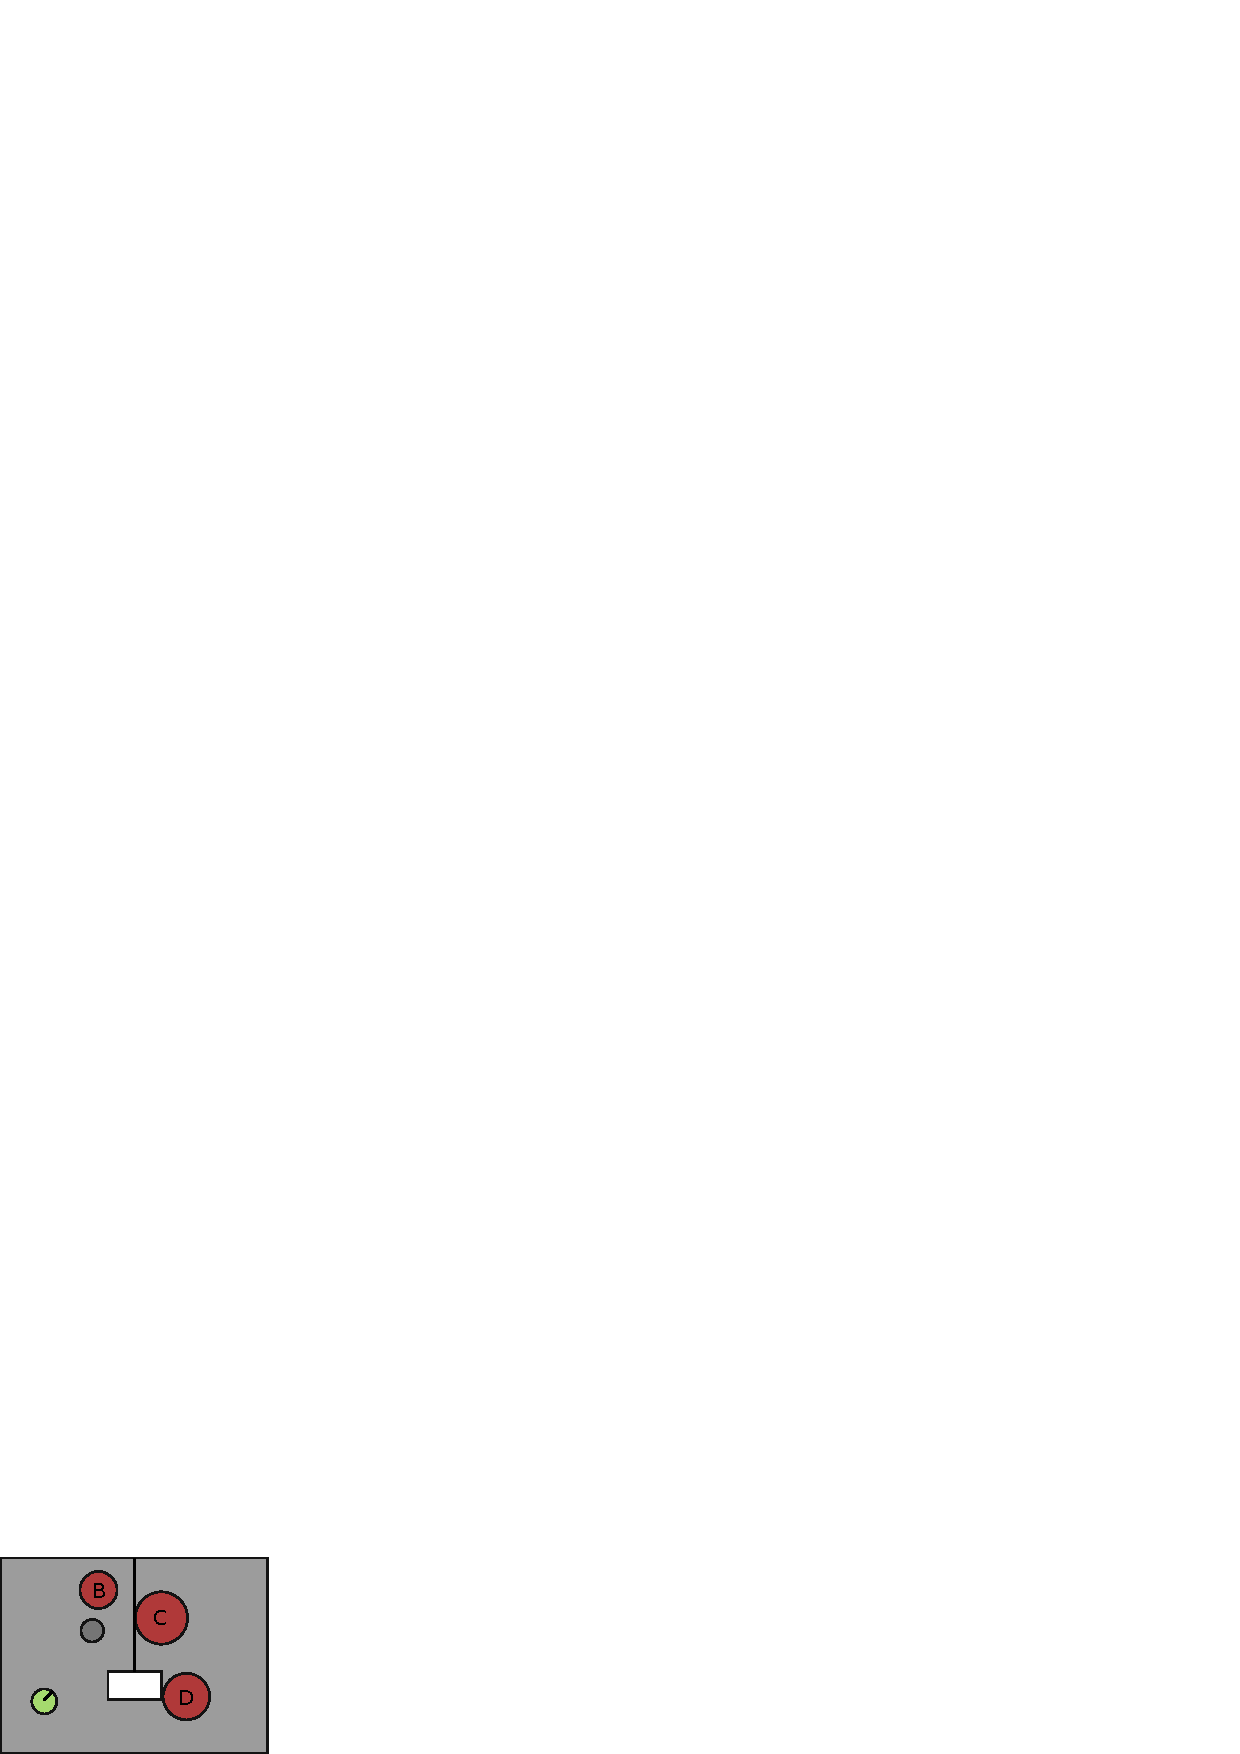
\includegraphics[width=.5\textwidth]{drawings/masked_map.pdf}
\end{wrapfigure}

Before diving into \cw{R\_DrawMasked} function, let's take the example of a simple room containing all types of "masked" elements and reexamine what needs to be done.\\
\par
The diagram shows a room with four walls (\cw{A}, \cw{B}, \cw{C}, and \cw{D}), a pillar also made of four walls (\cw{E}, \cw{F}, \cw{G}, and \cw{H}), a transparent wall \cw{I}, a barrel (in grey), a player spawn point (in green) and three enemies (in red: a Baron of Hell, a Cacodemon, and a Demon).\\
\par
The result as rendered by \doom{} is visible in figure \ref{masked.png}. Notice how the Baron is drawn on top of wall \cw{I}, the Cacodemon is partially occluded by wall \cw{I}, and parts of the demon are completely clipped behind the pillar. Also notice how the barrel must be drawn in front of the Baron for correctness. Last, wall \cw{I} needs to be clipped against the pillar.\\
\par
\cfullimage{masked.png}{Scene with all Things and the transparent wall rendered}
\par
With the desired result in mind, let's go back to where we were with only walls and flats rendered in the framebuffer. In the case of the same room, it would look like figure \ref{masked_nomasked.png}.\\
\par
\cfullimage{masked_nomasked.png}{Same scene as it is currently stored in the framebuffer}
\par
To get from figure \ref{masked_nomasked.png} to figure \ref{masked.png}, the engine needs to generate a list of maskables (also simply called sprites in the code), to sort them into back-to-front order, iterate over the sorted list, perform clipping on each of them, and finally render them as columns of pixels.\\
\par
\subsubsection{List Of Things}
 The list of things was built while the BSP was traversed. Each time a subsector was sent to rendering (in \cw{R\_Subsector}) the list of things it contained were added to an array of \cw{vissprite\_t}s. Note that things are only pseudo-ordered and therefore the order is not usable. In our example the barrel and the Baron would be added based on the subsector they were in, but in no precise order (in the subsector's list of things, the baron could be returned before the barrel).\\
 \par
 \subsubsection{Clipping Information}
 The clipping information was also built while rendering walls. Ideally it would have been a depth buffer but RAM was expensive and not fast enough. The solution was to record anything that could potentially appear on the screen in an optimized array of \cw{drawseg\_t}s.\\
\par

The "drawn segments" array \cw{drawsegs} is made of the following \cw{drawseg\_t} struct.\\
\par
\ccode{drawseg_t.c}\\
\par
It is not easy to understand at first but it is much easier to think of as a log of what occluders were rendered to the screen.
\begin{itemize} 
	\item For each wall that generated pixels in the framebuffer, a \cw{drawseg\_t} is added.
	\item For each portal, up to two \cw{drawseg\_t}s are added (one for the upper part and one for the lower part if the portal had no middle texture).
	\item For each masked segment (like the grid \cw{I} in our example) that was skipped, one \cw{drawseg\_t} entry is added to record what should have been drawn.
\end{itemize}
The log entries are ordered by distance from the player (since each entry was added while rendering the walls). The distance is not a \cw{z} value but a \cw{scale} value. The idea is to replay a portion of the log for each thing (everything in front of the thing) in order to build an accurate occlusion rectangle. Once the occlusion rectangle is obtained, the Thing is clipped against it. Each \cw{drawseg\_t} features the screen-space horizontal boundaries (\cw{x1} and \cw{x2}) as well as their respective scales (\cw{scale1} and \cw{scale2}). Since a scale value is generated for each Thing (based on its distance from the player), it is used to know what portion of the \cw{drawsegs} array to replay.\\
\par
The screen-space horizontal top and bottom edge of each wall are obtained from pointers \cw{sprtopclip} and \cw{sprbottomclip} which point to an array shared by all \cw{drawseg\_t}s.\\
\par
\ccode{openings.c} 
\par
\rawdrawing{openings_db}
\par
%Clearing the array of openings at the beginning of a frame is ridiculously simple, \cw{lastopening} only needs to be set to \cw{openings}.\\
Now that we know how they are clipped, let's take a look at how sprites are stored.\\
% \par
% The visible sprites (\cw{visprites}) storage is easier to understand than the \cw{drawseg\_t} array.\\
\par
\ccode{vissprites.c}
\par
A vissprite entry contains everything needed to render a sprite on screen. It features information similar to the drawn segments such as the screen space horizontal boundaries (\cw{x1} and \cw{x2}), its scale to compare distances with walls, the texture ID (\cw{patch}) and the lightlevel (\cw{colormap}) to be used for shading.\\
\par
Notice the \cw{prev} and \cw{next} fields. Even though vissprites are stored in a linear array, they need to be sorted into back-to-front order. Instead of moving around array elements, the sorting method only updates the doubly-linked list. This way, elements remain at the same array position but a sorted list can be obtained by following the \cw{next} pointers.
\newpage





Let's finally look at how all this data is used to render the sprites and masked segments in \cw{R\_DrawMasked}.\\
\par
\ccode{R_DrawMasked.c}\\
\par
As expected, the list of visible sprites is sorted based on their distances to the player (\cw{R\_SortVisSprites}). This process is fast since only \cw{scale} has to be compared and no data is copied into the array, the doubly-linked list is only updated to move an element.\\
\par
Next, all sprites are rendered one-by-one in a back-to-front fashion. The method taking care of this (\cw{R\_DrawSprite}) scans the array of \cw{drawseg}s linearly to find what wall fragments were drawn in front of the sprite and clips it accordingly. Since the search is based on the scale of each \cw{drawseg\_t} and the screen-space \cw{X} boundaries it is a fast operation.\\
\par
The last step is to render the masked segments which were skipped during BSP traversal. This is done in function \cw{R\_RenderMaskedSegRange}.\\
\par 
As explained earlier (render all sprites then render all masked segments), there is no way the grid in figure \ref{masked.png} could be interleaved with the sprites. To address this, there is a little "hack" in \cw{R\_DrawSprite} during the linear scan for occluding \cw{drawseg\_t}s. It detects which segments were "masked" and renders them via \cw{R\_RenderMaskedSegRange}.\\
\pagebreak



\subsection{Drawing Masked Player}
The last piece to render is the easiest of all. The sprite representing the Doomguy, a.k.a "the player sprite" (\cw{psprite}), is drawn on top of everything. There is no clipping in effect here, only the need to account for the lightmap induced by the sector the player is currently standing in and making the hand bob left and right when moving/running. Like other masked elements this sprite is rendered vertically as columns of pixels.\\
\par
You may have noticed in \cw{R\_DrawMasked} that the player hand is drawn only if the viewing angle offset is equal to zero (\cw{viewangleoffset}). This is an artifact of a feature that was disabled in later versions. Until v1.2, \doom{} supported a "three screen mode" where three computers with three monitors could be networked to render a wide field of view.\\
\par
\fullimage{three_screens_mode.png}
\par
It is likely John Carmack was inspired to add this feature when he visited Alaska Airline training center, where he was able to see a multi-million dollar wide-screen flight simulator\footnote{Source: "http://leeland.stores.yahoo.net/earlydoomstuff.html"}. The feature was cut in later versions. \\
\par
\trivia{Only the command-line code to enable/disable multiple screens was removed, the feature itself remained. Chocolate \doom{} re-enabled it and even created a special mode allowing the "three monitor view" to be experienced on a single machine. This is how the above screenshot was created.}\\
\par
% \trivia{Player has gloves when handling most weapons but he takes them off when using the point american.}\\

\vspace{-10pt}
\subsection{Picture format}
Sprites are written one vertical column at a time but are stored in a way that cuddles the i486 cachelines during read operations. Each sprite is stored in its own lump and consists of a collection of lines describing the vertical columns in the sprite (in essence, sprites are stored rotated 90 degrees counterclockwise).\\
\par
Each column (also called "post" in the code) is a set of "spans" with one byte giving the vertical offset where the span starts, then one byte giving the size of the payload and finally the texel payload.
\pagebreak


\fullimage{sprite_format.png}\\
\par
The Lost Soul sprite's row \cw{44} is 4 bytes (one span with: \cw{0x13} vertical offset, \cw{0x02} data length, \cw{0x54} and \cw{0x59} two texels). Row \cw{33} has two spans, accounting for 48 bytes and is a rare case where the encoding scheme is less favorable than "uncompressed" which would have been 47 bytes. Row \cw{10} (also two spans) accounts for 19 bytes which is much less than the uncompressed length of 47 bytes. This entire Lost Soul sprite is 44x47 and fits in 1360 bytes for a surface of 2068 pixels, resulting in a rough 50\% compression ratio.\\
\par
\vspace{-10pt}
\subsection{Sprite aspect ratio}
The framebuffer was distorted when transfered from the VGA hardware to the CRT screen. The different aspect ratios make pixels taller than they are wide, stretching images vertically.\\
\par
This distortion had not been an issue when working with Deluxe Paint since the tool could be set up in 320x200 (so artists did not have square pixels) but it was something to factor in when id switched to using scanned images from the NextDimension.




\cfullimage{sprites_ratio_demon.png}{Demon storage vs rendered}
\par
\vspace{-5pt}
The Cacodemon was purposely drawn and rendered elliptically but effectively stored as a rounded shape. In the early days of tool authoring, programmers of asset extractors did not account for the CRT distortion, resulting in bulky monster visuals\footnote{Even toy manufacturers made the mistake. Reaper Miniatures' Cacodemon figurine is round instead of elliptic.}.\\
\par
\vspace{-5pt}
{
\setlength{\belowcaptionskip}{-10pt}
\cfullimage{sprites_ratio_cacodemon.png}{Cacodemon storage vs rendered}
}
